%\documentclass{beamer}
\documentclass{ctexbeamer} 
\definecolor{GreenDarkFaded}{rgb}{0,0.6,0}
\definecolor{SpringGreenDark}{rgb}{0.2,0.6,0}
\definecolor{GreenObscureWeak}{rgb}{0,0.2,0}
\definecolor{GreenDarkDull}{rgb}{0.2,0.6,0.2}
\mode<presentation>
{
 % \usetheme{PaloAlto}
 \usetheme{Warsaw}
 % \usetheme{Darmstadt}
 % \usetheme{Boadilla}
 \usecolortheme{orchid}
 %\usecolortheme[named=GreenDarkDull]{structure}
 % \usecolortheme{orchid}
 % \usecolortheme{whale}
 % \usecolortheme{default}
 % \usecolortheme{wolverine}
 % \usecolortheme{crane}
 % \usecolortheme{rose}
 \setbeamercovered{transparent}
}

% \usepackage{pdfpages}
% \includepdf{demo.pdf}  % 插入pdf文件 
% \usepackage{navigator}
% \embeddedfile[TeX code]{\jobname}{\jobname.tex}  % 插入tex文件
% \usepackage{attachfile}
% \attachfile{demo.pdf}

\usepackage[english]{babel}
\usepackage[utf8]{inputenc}
% \usepackage{times}
% \usepackage[T1]{fontenc}
\usepackage{graphicx} %图片
\usepackage{booktabs} %表格


%Information to be included in the title page:
\title[光伏发电预测]{基于深度学习的光伏发电量预测方法的实现与分析}
\author{汇报人:xxx \newline  指导老师:xxx}
\institute{xxx}
\date{2023年3月10日}

\begin{document}
\begin{frame}
  \titlepage
\end{frame}


\begin{frame}{目录}

    \tableofcontents     %与上面的函数对应,该命令是自动生成包含章节标题和对应页码的目录表
  
\end{frame}

\AtBeginSection[]{
	\begin{frame}
		\tableofcontents[currentsection]
	\end{frame}
} % 每到新的一节(Section)显示大纲

% \AtBeginSubsection[]{
% 	\begin{frame}
% 		\frametitle{目录}
% 		\tableofcontents[currentsubsection]
% 	\end{frame}
% }


\graphicspath{{figures/}}

\section{Motivation}
\subsection{Why We Need PV}
%\subsection{Why We Need to Predict}

    \begin{frame}{Why We Need PV}{光伏新能源}
        \begin{itemize}
        \item
        太阳能已迅速成为许多国家日益重要的能源。光伏发电数据是典型的时间序列,具有趋势和周期性。
        \item
        在与全球变暖作斗争中,发展可再生能源已成为各国共同努力的目标.光伏(PV)是最受欢迎的可再生能源之一,因为它环保,无限且具有成本效益.
        \end{itemize}
    \end{frame}



\subsection{Why We Need to Predict}
    \begin{frame}{Why We Need to Predict}{间断,不连续,波动大}
        \begin{itemize}
        \item
        光伏发电间歇性的性质和与预测相关的不确定性是必须克服的难题,以保持电力系统的稳定性。
        \item
        虽然储能设备可以节省过多的能源用于周转,但其高成本并不适合大多数用户。因此,光伏发电的准确预测对于工业应用变得非常重要。
        \end{itemize}
    \end{frame}




\section{Related Work}
\subsection{Physical Methods}

    \begin{frame}{物理方法}{数值预报,微分方程}
        \begin{itemize}
        \item
        是对表现最佳的全球数值天气预报(NWP)模型的气象输出的后处理。
        \item
        固定时间间隔地处理来自5个地球静止气象卫星的卫星图像。
        \item
        利用实时卫星数据预测近期的云运动,然后应用卫星到辐照度模型来计算全球水平和平面内辐照度.云运动矢量(CMV)模型从最近的历史到当前时间到未来10天的太阳能和光伏数据。
        \end{itemize}
    \end{frame}

\subsection{Statistic Methods}
    \begin{frame}{统计方法}{ARIMA}
        \begin{itemize}
        \item 
        自回归模型:AR
        \begin{equation}
            y_t = \mu + \sum_{i=1}^{p}\gamma_i y_{t-i} + \epsilon_t
        \end{equation}

        \item 
        移动平均模型:MA
        \begin{equation}
            y_t = \mu + \sum_{i=1}^{p}\theta_i \epsilon_{t-i} + \epsilon_t
        \end{equation}

        \item 
        自回归移动平均模型:ARMA
        \begin{equation}
            y_t = \mu + \sum_{i=1}^{p}\gamma_i y_{t-i} + \sum_{i=1}^{p}\theta_i \epsilon_{t-i} + \epsilon_t
        \end{equation}

        \end{itemize}

    \end{frame}

\subsection{Deep Learning Methods}
    \begin{frame}{深度学习}{LSTM}
        \begin{columns}
            \column{0.8\textheight}
            \begin{block}{Mathematics}
            \begin{center}
            \begin{gather*}
                f_t = \sigma (W_f [h_{t-1},x_t] + b_f)\\
                i_t = \sigma (W_i [h_{t-1},x_t] + b_i)\\
                \tilde{C_t} = tanh(W_c [h_{t-1},x_t] + b_c)\\
                C_t = f_t * C_{t-1} + i_t * \tilde{C_t}\\
                o_t = \sigma (W_o [h_{t-1},x_t] + b_o)\\
                h_t = o_t * tanh(C_t)
            \end{gather*} 
            \end{center} 
            \end{block}
            \column{0.5\textwidth}
            \begin{figure}
                \centering
                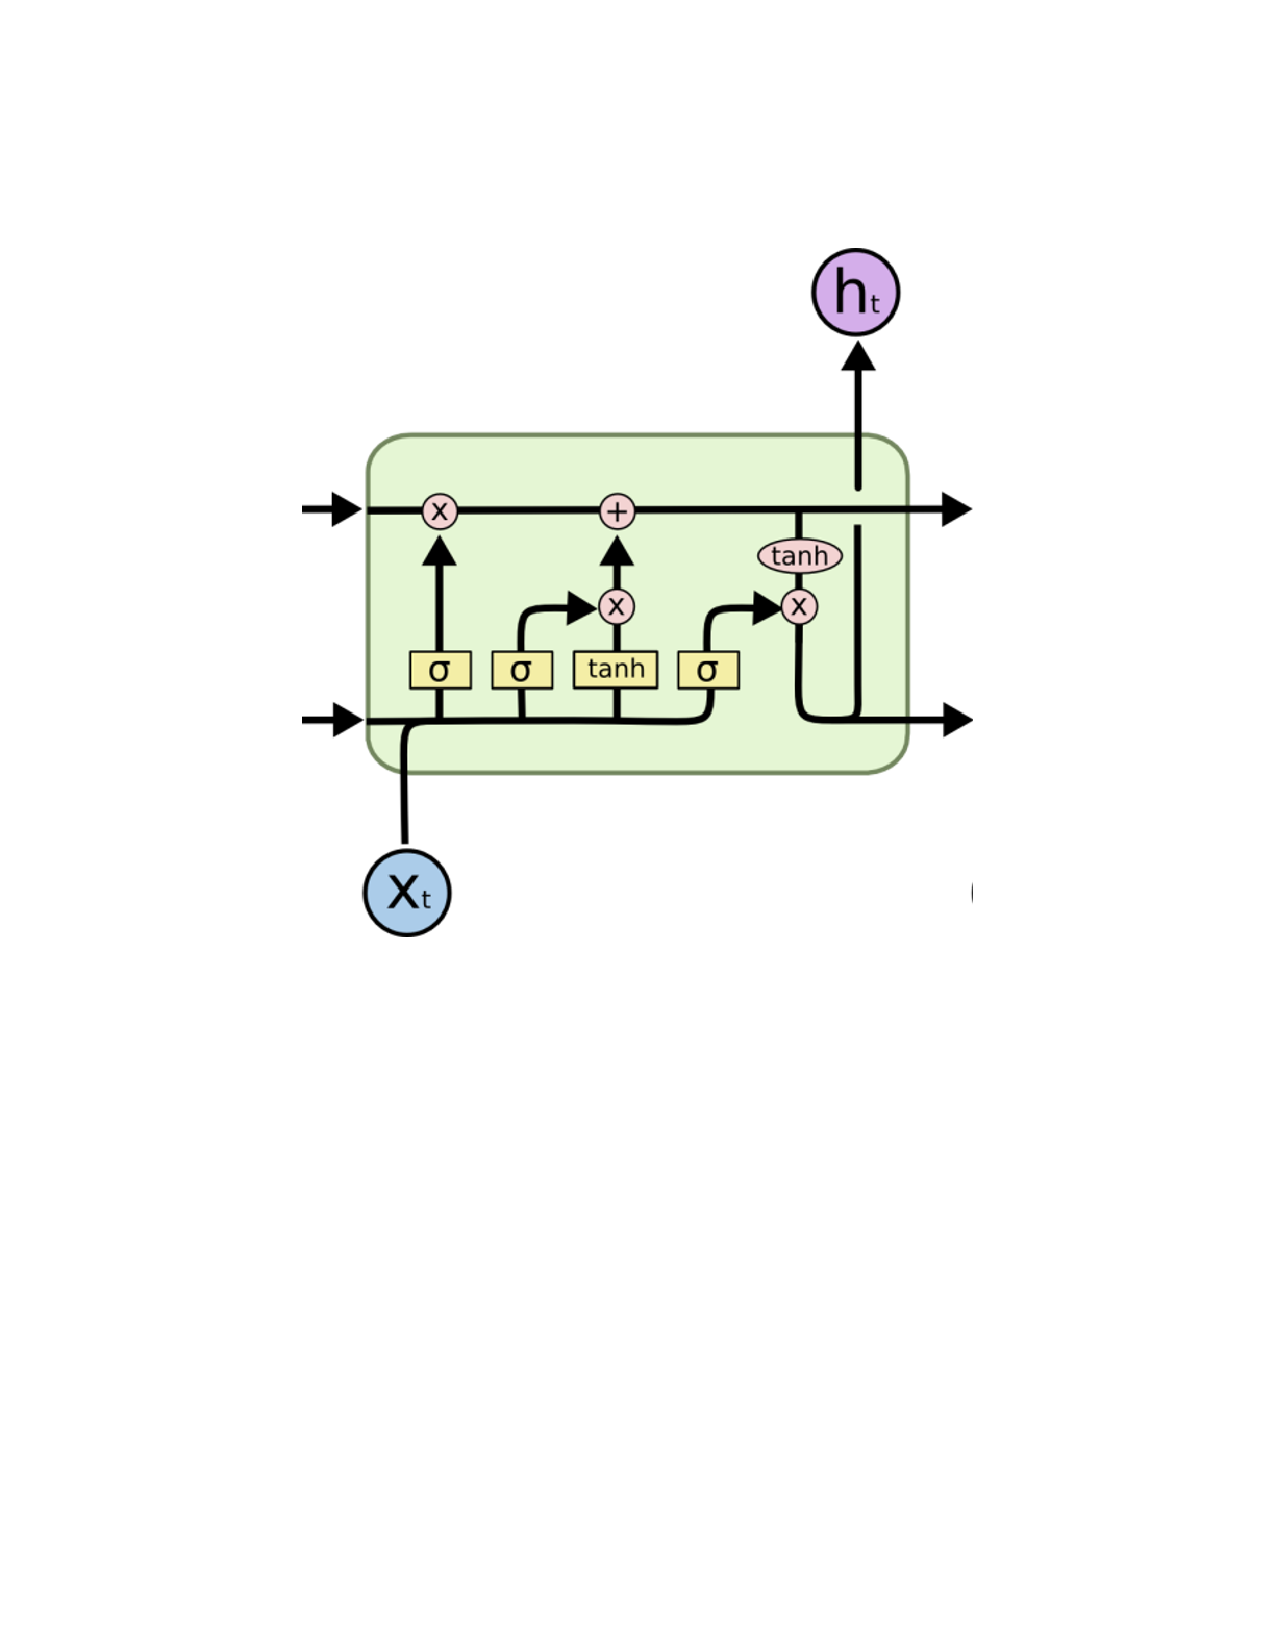
\includegraphics[width=6cm]{LSTM.pdf}
                % \caption{LSTM}
                % \label{LSTM_Cell_figures}
            \end{figure}
        \end{columns}
    \end{frame}

\section{My Methods and Methodology}
\subsection{dataset}
\begin{frame}{数据集}{浙江台州光伏传感器}
如表\ref{tab1}所示
\begin{table}
\centering
\caption{Dataset}
\label{tab1}
\begin{tabular}{cccccc}
\toprule
时间戳 & 发电量 & 直流电流 & 逆变器温度 & 天气  \\
\midrule
2021-4-1 00:00:00 & 0 & 0 & 18 & 晴   \\
2021-4-1 01:00:00 & 99 & 100 & 50 & 晴  \\
2021-4-1 02:00:00 & 128 & 100 & 50 & 晴 \\
...               & ... & ... & ... & ... \\
2022-12-30 23:00:00 & 0 & 0 & 20 & 小雨 \\
\bottomrule
\end{tabular}
\end{table}
15000 rows-5 cols
\end{frame}

\subsection{Review of Model}
\begin{frame}{模型综述}{Patch-LSTM}

    \begin{columns}
        \column{0.4\textwidth}
        \begin{itemize}
            \item {模型输入:光伏发电量的历史数据(24h,48h,72h),天气信息,逆变器温度,直流电流}
            \item {模型结构:维度变换,特征提取(CNN,LSTM),信息融合(MLP)}
            \item {模型输出:未来24小时的发电量}
        \end{itemize}

        \column{0.6\textwidth}
            \begin{center}
                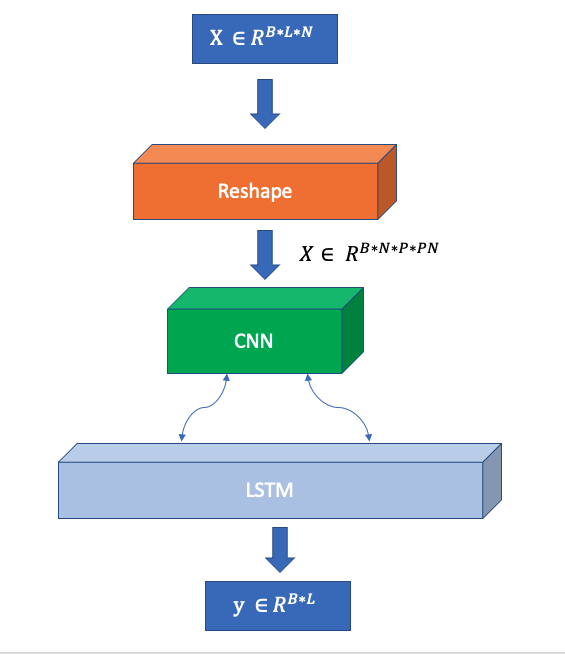
\includegraphics[width=4.5cm]{模型架构}
            \end{center}
    \end{columns}
\end{frame}

\subsection{Details of Model}
\begin{frame}{维度转换}{Dimention Transformation}
    \begin{columns}
        \column{0.5\textwidth}
        \begin{center}
            \begin{block}{Formula:}
                \begin{equation*}
                    B*N*L = B*N*P*PN
                \end{equation*}

            \end{block}   
        \end{center}
        \column{0.5\textwidth}
            \begin{figure}
                \centering
                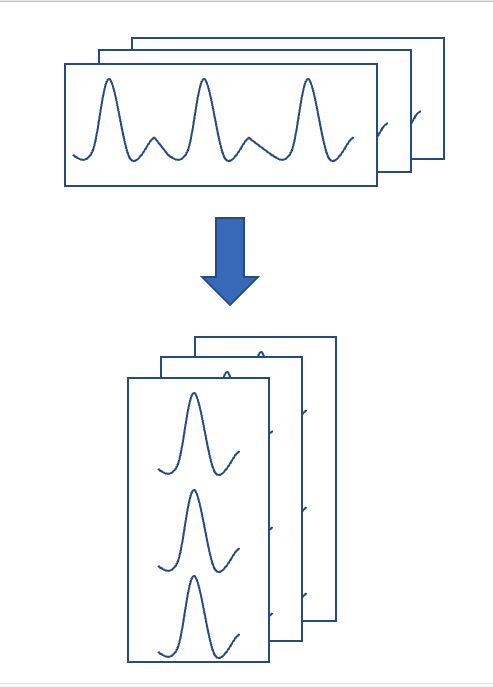
\includegraphics[width=4.5cm]{维度变换}
                %\caption{LSTM}
                % \label{LSTM_Cell_figures}
            \end{figure}
    \end{columns}
\end{frame}

\begin{frame}{局部信息提取}{Extract Local Information}
    通过一个固定大小的感受野随着时间维度进行滑动,提取局部信息
    \begin{center}
        \begin{block}{Mathematics}
        \begin{equation*}
            C_t = W_{t-1}X_{t-1}+W_t X_t+W_{t+1}X_{t+1}
        \end{equation*}
        \end{block}
    \end{center}
    \begin{center}
    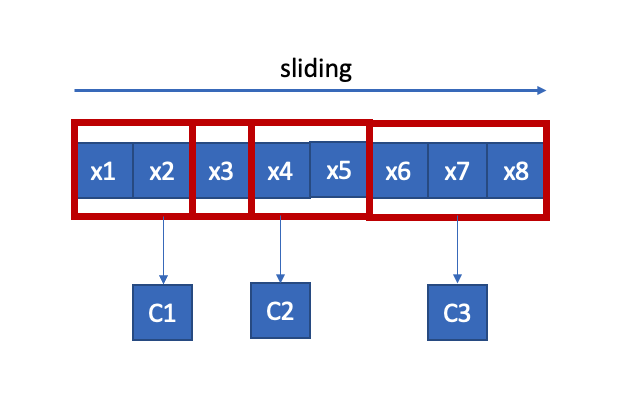
\includegraphics[width=6cm]{Conv1d}
    \end{center}
\end{frame}

\begin{frame}{时序信息提取}{Extract Temporal Information}
    通过LSTM循环神经网络,提取时序信息。
    \begin{columns}
        \column{0.6\textwidth}
        \begin{center}
        \begin{block}{Mathematics}
        \begin{center}
        \begin{gather*}
            f_t = \sigma (W_f [h_{t-1},x_t] + b_f)\\
            i_t = \sigma (W_i [h_{t-1},x_t] + b_i)\\
            \tilde{C_t} = tanh(W_c [h_{t-1},x_t] + b_c)\\
            C_t = f_t * C_{t-1} + i_t * \tilde{C_t}\\
            o_t = \sigma (W_o [h_{t-1},x_t] + b_o)\\
            h_t = o_t * tanh(C_t)
        \end{gather*} 
        \end{center} 
        \end{block}
        \end{center}
        \column{0.6\textwidth}
        \begin{figure}
            \centering
            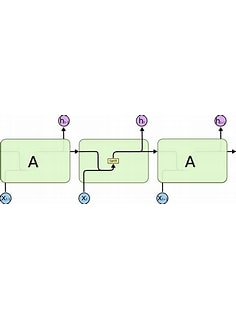
\includegraphics[width=5cm]{lstm}
            % \caption{LSTM}
            % \label{LSTM_Cell_figures}
        \end{figure}
    \end{columns}
\end{frame}

\subsection{Experiment}
\begin{frame}{实验}{指标,对比模型,预期结果}
\begin{itemize}
    \item {指标:平均绝对百分比误差(Mean Absolute Percentage Error)}
    \begin{center}
        \begin{equation*}
            MAPE = \frac{100\%}{n} \sum_{i=1}^{n}|\frac{\hat{y_i}-y_i}{y_i}|
        \end{equation*}
    \end{center}  
    \item {对比模型:}
    \begin{itemize}
        \item {Informer}
        \item {Autoformer}
    \end{itemize}
    \item {预期结果:}
    \begin{itemize}
        \item {MAPE低于20\%的天数占比50\%以上}
    \end{itemize}
\end{itemize}
\end{frame}

\section{Summary}
\begin{frame}{时间安排}{Timeline}
    如表\ref{tab2}所示
    \begin{table}
    \centering
    \caption{Dataset}
    \label{tab2}
    \begin{tabular}{cccccc}
    \toprule
    序号 & 时间 & 内容  \\
    \midrule
    1 & 2022.12.20-2023.1.7 & 查询相关资料并熟悉课题  \\
    2 & 2023.1.8-2023.1.12 & 任务书  \\
    3 & 2023.3.6-2023.3.12 & 开题报告  \\
    4 & 2023.3.19-2023.4.1 & 研究具体方案,搭建程序框架  \\
    5 & 2023.4.2-2023.4.15 & 进行实验分析  \\
    6 & 2023.4.16-2023.4.29 & 改进深度学习模型  \\
    7 & 2023.4.30-2023.5.13 & 期中检查并撰写毕业论文  \\
    8 & 2023.5.24-2023.5.30 & 论文评审及查重  \\
    10 & 2023.6.4-2023.6.10 & 答辩报告会  \\
    \bottomrule
    \end{tabular}
    \end{table}
\end{frame}




\begin{frame}
    \begin{center}
        汇报完毕~~~~恳请指正
        ~\\
        ~\\
        ~\\
        ~\\
        ~\\
        Presented by
        ~\\
        xxx
    \end{center}
\end{frame}




\end{document}